\documentclass{article}[18pt]
\ProvidesPackage{format}
%Page setup
\usepackage[utf8]{inputenc}
\usepackage[margin=0.7in]{geometry}
\usepackage{parselines} 
\usepackage[english]{babel}
\usepackage{fancyhdr}
\usepackage{titlesec}
\hyphenpenalty=10000

\pagestyle{fancy}
\fancyhf{}
\rhead{Sam Robbins}
\rfoot{Page \thepage}

%Characters
\usepackage{amsmath}
\usepackage{amssymb}
\usepackage{gensymb}
\newcommand{\R}{\mathbb{R}}

%Diagrams
\usepackage{pgfplots}
\usepackage{graphicx}
\usepackage{tabularx}
\usepackage{relsize}
\pgfplotsset{width=10cm,compat=1.9}
\usepackage{float}

%Length Setting
\titlespacing\section{0pt}{14pt plus 4pt minus 2pt}{0pt plus 2pt minus 2pt}
\newlength\tindent
\setlength{\tindent}{\parindent}
\setlength{\parindent}{0pt}
\renewcommand{\indent}{\hspace*{\tindent}}

%Programming Font
\usepackage{courier}
\usepackage{listings}
\usepackage{pxfonts}

%Lists
\usepackage{enumerate}
\usepackage{enumitem}

% Networks Macro
\usepackage{tikz}


% Commands for files converted using pandoc
\providecommand{\tightlist}{%
	\setlength{\itemsep}{0pt}\setlength{\parskip}{0pt}}
\usepackage{hyperref}

% Get nice commands for floor and ceil
\usepackage{mathtools}
\DeclarePairedDelimiter{\ceil}{\lceil}{\rceil}
\DeclarePairedDelimiter{\floor}{\lfloor}{\rfloor}

% Allow itemize to go up to 20 levels deep (just change the number if you need more you madman)
\usepackage{enumitem}
\setlistdepth{20}
\renewlist{itemize}{itemize}{20}

% initially, use dots for all levels
\setlist[itemize]{label=$\cdot$}

% customize the first 3 levels
\setlist[itemize,1]{label=\textbullet}
\setlist[itemize,2]{label=--}
\setlist[itemize,3]{label=*}

% Definition and Important Stuff
% Important stuff
\usepackage[framemethod=TikZ]{mdframed}

\newcounter{theo}[section]\setcounter{theo}{0}
\renewcommand{\thetheo}{\arabic{section}.\arabic{theo}}
\newenvironment{important}[1][]{%
	\refstepcounter{theo}%
	\ifstrempty{#1}%
	{\mdfsetup{%
			frametitle={%
				\tikz[baseline=(current bounding box.east),outer sep=0pt]
				\node[anchor=east,rectangle,fill=red!50]
				{\strut Important};}}
	}%
	{\mdfsetup{%
			frametitle={%
				\tikz[baseline=(current bounding box.east),outer sep=0pt]
				\node[anchor=east,rectangle,fill=red!50]
				{\strut Important:~#1};}}%
	}%
	\mdfsetup{innertopmargin=10pt,linecolor=red!50,%
		linewidth=2pt,topline=true,%
		frametitleaboveskip=\dimexpr-\ht\strutbox\relax
	}
	\begin{mdframed}[]\relax%
		\centering
		}{\end{mdframed}}



\newcounter{lem}[section]\setcounter{lem}{0}
\renewcommand{\thelem}{\arabic{section}.\arabic{lem}}
\newenvironment{defin}[1][]{%
	\refstepcounter{lem}%
	\ifstrempty{#1}%
	{\mdfsetup{%
			frametitle={%
				\tikz[baseline=(current bounding box.east),outer sep=0pt]
				\node[anchor=east,rectangle,fill=blue!20]
				{\strut Definition};}}
	}%
	{\mdfsetup{%
			frametitle={%
				\tikz[baseline=(current bounding box.east),outer sep=0pt]
				\node[anchor=east,rectangle,fill=blue!20]
				{\strut Definition:~#1};}}%
	}%
	\mdfsetup{innertopmargin=10pt,linecolor=blue!20,%
		linewidth=2pt,topline=true,%
		frametitleaboveskip=\dimexpr-\ht\strutbox\relax
	}
	\begin{mdframed}[]\relax%
		\centering
		}{\end{mdframed}}
\lhead{Networks and Systems - Networks}


\begin{document}
\begin{center}
\underline{\huge Physical Layer}
\end{center}
\section{Bandwidth}
Bandwidth is the physical property fo the transmission medium
\begin{defin}[Baseband]
	The signal that runs from 0 to a maximum frequency. Has very narrow and near-zero frequency range. Used in wires
\end{defin}
\begin{defin}[Passband]
	Signals that occupy the higher range of frequency and pass through frequency filter(s). Used in wireless spectrum
\end{defin}
\subsection{Signal Bandwidth}
Bandwidth of analogue and digital signals are measured differently:
\begin{itemize}
	\item Analogue signal bandwidth is measured in terms of its frequency (Hz)
	\item Digital signal bandwidth is measured in terms of bit rate (bps)
\end{itemize}
\section{Digital Modulation}
Digital signals (0,1) are encoded by low and high voltage\\
\\
There are many digital encoding schemes
\begin{center}
	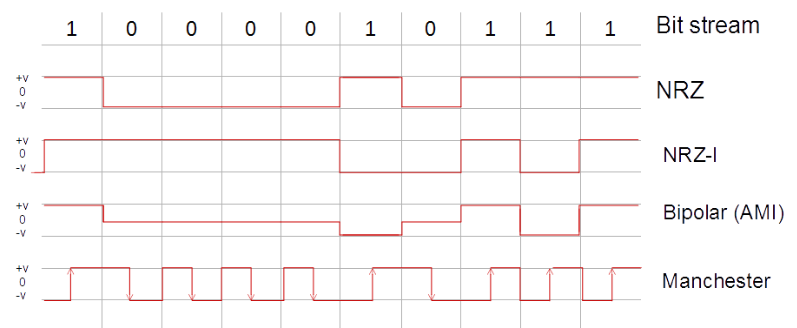
\includegraphics[scale=0.7]{Modulation}
\end{center}
\subsection{NRZ Encoding (Non-Return-to-Zero)}

\begin{defin}[NRZ Encoding]
\begin{itemize}
	\item A high voltage represents a 1 and a low voltage represents a 0
	\item The voltage does not return to zero, it changes only when the bit value changes
\end{itemize}
\end{defin}




\begin{itemize}
	\item Problem: having long runs of consecutive bits with the same value (no changes in voltage) the constant signal values can't synchronize the communicating devices
	\item Especially with long runs of either 0 or 1, there is no change to resynchronise so it is likely that the clocks would get out of sync
\end{itemize}
\subsection{NRZI Encoding}
\begin{itemize}
	\item NRZI attempts to alleviate the problem in NRZ scheme
\end{itemize}
\begin{defin}[NRZI Encoding]
\begin{itemize}
	\item 0 is encoded as no change in the level. 1 is encoded depending on the current state of the line
	\item 1 is encoded as an inverting of the current state
\end{itemize}
\end{defin}


\begin{itemize}
	\item This fixes the problem of sending consecutive 1s but not consecutive 0s
\end{itemize}
\subsection{Bipolar Encoding}
\begin{defin}[Bipolar Encoding]
\begin{itemize}
	\item 0 is represented by a zero voltage, neither high nor low
	\item 1 is represented by either positive voltage or negative voltage
	\begin{itemize}
		\item It is inverted based on the last transmission of 1
		\item It is represented by a negative voltage if it was represented by a positive voltage when it was last transmitted, and vice versa
	\end{itemize}
\end{itemize}
\end{defin}
For this, over a long enough message, the sum of the voltages is zero, this is called a "balanced encoding" and is desirable in some applications

\subsection{Manchester Encoding}
\begin{defin}[Manchester Encoding]
\begin{itemize}
	\item A high to low voltage represents a 1 and a low to high voltage represents a 0
	\item Uses signal changes to transmit a bit and achieves synchronisation
	\item This is equivalent to an XOR of the clock signal and the NRZ encoding. The clock is at twice the frequency of the NRZ
\end{itemize}
\end{defin}
\begin{itemize}
	\item Twice the bandwidth of NRZ is required
\end{itemize}
\section{Multiplexing}
\begin{itemize}
	\item Channels are often shared by multiple signals
	\item Different ways to accomplish multiplexing:
\end{itemize}
\subsection{Frequency Division Multiplexing}
\begin{itemize}
	\item Refactor the signals to start at different frequencies
	\item Sit them side by side on the frequency spectrum on the same channel, so they don't interfere with each other
	\item Put a small region in-between adjacent frequency bands to avoid interference
\end{itemize}
\begin{center}
	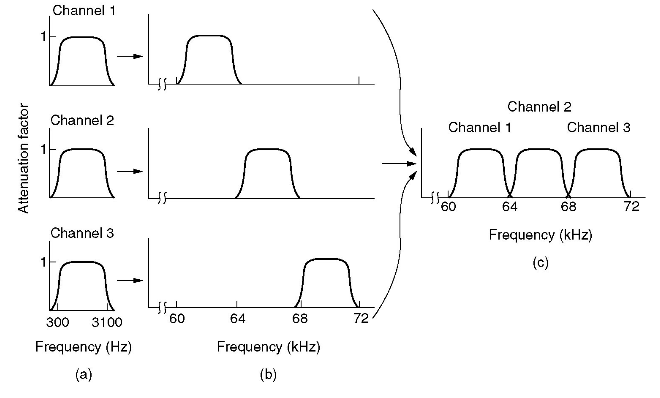
\includegraphics[scale=0.7]{FDM}
\end{center}
\begin{enumerate}[label=\alph*]
	\item The original bandwidths
	\item The bandwidths raised in frequency
	\item The multiplexed channel
\end{enumerate}
\subsection{Wavelength Division Multiplexing}
\begin{itemize}
	\item The same as FDM but for optical fibres instead of wireless signals
\end{itemize}
\begin{center}
	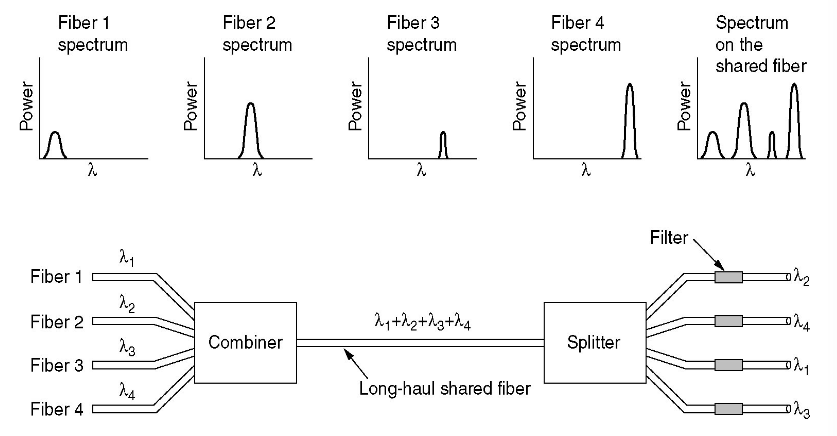
\includegraphics[scale=0.7]{WDM}
\end{center}
\subsection{Time division multiplexing}
\begin{itemize}
	\item Intersperse the channels in some sequence, leave a guard time to be able to separate out information
\end{itemize}
\begin{center}
	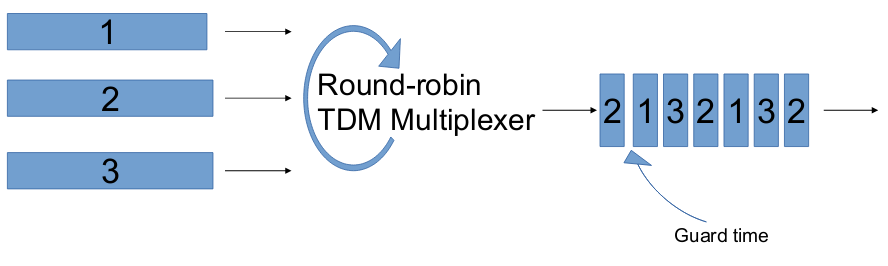
\includegraphics[scale=0.7]{TDM}
\end{center}
\subsection{Code Division Multiple Access}
\begin{itemize}
	\item Nice and clean mathematical method allows every transmitter to use the entire channel all the time
	\item The individual transmissions are blended (or extracted by a receiver) using coding theory
	\item Imagine that we have four transmitters called, from now on, stations
	\item Each station has a chip (i.e. a code), which is a four bit vector
	\item These codes are chosen so that the dot product of any of these codes with any other of the codes is 0 i.e. they are orthogonal to each other
	\item Transmitting the stations chip sequence a 1
	\item Transmitting the negation of a stations chip sequence is a 0
\end{itemize}


\end{document}